\documentclass[runningheads]{llncs}
\usepackage{graphicx}
\usepackage{hyperref}
\usepackage{amsmath}
\usepackage{amsfonts}
\usepackage{listings}
\usepackage{xcolor}
\usepackage{float}
\usepackage{booktabs}
\usepackage{tikz}
\usetikzlibrary{shapes,arrows,positioning}

\title{Retrieval-Augmented Generation for Cirq Quantum Code Generation: A Multi-Agent, Tool-Augmented Approach}
\titlerunning{RAG for Cirq Quantum Code Generation}

\author{Umer Farooq \and Hussain Waseem Syed \and Muhammad Irtaza Khan}
\institute{FAST NUCES Islamabad, Department of Computer Science\\
\email{i220891@nu.edu.pk, i220893@nu.edu.pk, i220911@nu.edu.pk}}

% Custom spacing to tighten layout around floats
\setlength{\textfloatsep}{12pt plus 2.0pt minus 2.0pt}  % Space between top/bottom float and text
\setlength{\floatsep}{8pt plus 2.0pt minus 2.0pt}      % Space between two consecutive floats
\setlength{\intextsep}{12pt plus 2.0pt minus 2.0pt}    % Space around an in-text float

\begin{document}
\maketitle

\begin{abstract}
We present a specialized Retrieval-Augmented Generation (RAG) system for generating accurate Cirq quantum computing code from natural language descriptions. Our approach combines a curated knowledge base of Cirq implementations with a multi-agent Large Language Model (LLM) framework to produce executable quantum circuits with comprehensive explanations. The system addresses the growing need for accessible quantum programming tools by providing an AI-powered assistant specifically tailored for Google's Cirq framework. We evaluated our approach using standard quantum algorithms including VQE, QAOA, and quantum teleportation, achieving over 90\% syntactically correct code generation with distinct improvements over baseline LLM-only approaches. Our system leverages a novel combination of Designer, Optimizer, Validator, and Educational agents to ensure high-quality, educationally valuable output.
\keywords{Retrieval-Augmented Generation \and Cirq \and Quantum Computing \and Code Generation \and Educational AI \and Multi-Agent Systems \and Tool-Augmented LLMs}
\end{abstract}

\section{Introduction}

Quantum computing represents a paradigm shift in computational capabilities, promising exponential speedups for specific problems. However, the steep learning curve associated with quantum programming frameworks presents a significant barrier to adoption. Google's Cirq framework, while powerful, requires deep understanding of quantum mechanics and Python programming, making it challenging for newcomers to the field.

The complexity of quantum programming is compounded by the need to understand both quantum mechanical principles and framework-specific syntax. Traditional approaches to learning quantum programming rely heavily on documentation and examples, which can be overwhelming for beginners. This creates a significant gap between theoretical understanding and practical implementation.

Recent advances in Large Language Models (LLMs) and Retrieval-Augmented Generation (RAG) systems offer promising solutions to this challenge \cite{siavash2025modeldrivenquantumcodegeneration}. RAG systems combine the generative capabilities of LLMs with external knowledge bases, enabling more accurate and contextually relevant responses. 

Our work introduces a specialized RAG system for Cirq quantum code generation that addresses these challenges through a curated knowledge base and intelligent retrieval mechanisms. The system is designed to serve both educational and practical purposes, aiming to help users learn quantum programming while generating production-ready code. Our contribution involves a Multi-Agent architecture comprising Designer, Optimizer, Validator, and Educational agents that collaborate to generate, refine, and explain quantum circuits.

\section{Related Work}

\subsection{Quantum Code Generation}
Recent work has explored the application of AI to quantum programming. Dupuis et al. \cite{10691762} present the Qiskit Code Assistant, demonstrating framework-specific training. Similarly, Jimenez-Navajas et al. \cite{jimenez2025codegeneration} explore code generation for classical-quantum systems. Siavash and Moin have also contributed significantly with LLM-powered transpilation \cite{siavash2025llmpoweredquantumcodetranspilation}. Beyond framework-specific tools, standard language models trained on code have shown substantial capabilities in general code generation tasks, as demonstrated in seminal work like OpenAI Codex by Chen et al. \cite{chen2021evaluating}.

\subsection{Retrieval-Augmented Generation}
RAG systems have shown significant promise in improving the accuracy of LLM outputs. Siavash and Moin \cite{siavash2025modeldrivenquantumcodegeneration} present a model-driven approach to quantum code generation using RAG. We build on this by incorporating a multi-agent system. Originally introduced by Lewis et al. \cite{lewis2020retrieval} to enhance language models on knowledge-intensive NLP tasks, RAG has since been adapted to software engineering and code generation to mitigate hallucinations and update local syntax conventions.

\subsection{Agents and Optimization}
Multi-agent systems and fine-tuning are becoming central to quantum software engineering. Campbell et al. \cite{campbell2025enhancingllmbasedquantumcode} discuss enhancing generation with multi-agent optimization. Yu et al. \cite{yu2025quasarquantumassemblycode} introduce QUASAR for assembly generation via Agentic RL, while Jern et al. \cite{jern2025agentqfinetuninglargelanguage} explore fine-tuning for optimization. Our work integrates these concepts into a unified Cirq-specific pipeline. Furthermore, multi-agent architectures that incorporate iterative validation and testing loops—such as AgentCoder by Chen et al. \cite{chen2023agentcoder}—have proven effective in correcting bugs and enhancing overall code quality before final execution.

\subsection{Educational AI Systems}
Basit et al. \cite{basit2025pennylangpioneeringllmbasedquantum} introduce PennyLang, emphasizing dataset curation for education. Our work follows similar methodologies for constructing a Cirq-centric educational knowledge base.

\section{Methodology}

\subsection{System Architecture}
Our system employs a hybrid RAG + Multi-Agent architecture orchestrated to emulate a human developer's workflow. The \texttt{Orchestrator} class manages a complex state machine that coordinates four specialized LLM agents. The entire system is driven by a central \texttt{config.json} file that controls agent behaviors, RAG parameters, and optimization targets.

The pipeline follows a strict execution flow (Fig.~\ref{fig:arch}):
\begin{enumerate}
    \item \textbf{Designer Agent}: Fetches relevant Cirq code from the RAG Knowledge Base and generates the initial circuit implementation.
    \item \textbf{Validator Agent (Initial Pass)}: Performs static analysis using the \texttt{CirqCompiler} tool. If validation fails, it uses an LLM to generate a fix and re-validates in a \textbf{self-correction loop} (up to 3 retries).
    \item \textbf{Optimizer-Validator Loop}: The Optimizer refines the circuit (reducing depth/gates) using Cirq heuristics (e.g., \texttt{merge\_single\_qubit\_gates\_to\_phxz}). The Validator immediately verifies the optimized code, and the loop continues until convergence.
    \item \textbf{Final Validation}: A rigorous final check to ensure correctness.
    \item \textbf{Educational Agent}: Generates comprehensive explanations with four depth levels: \texttt{low}, \texttt{intermediate}, \texttt{high}, and \texttt{very\_high}.
\end{enumerate}

\begin{figure}[H]
    \centering
    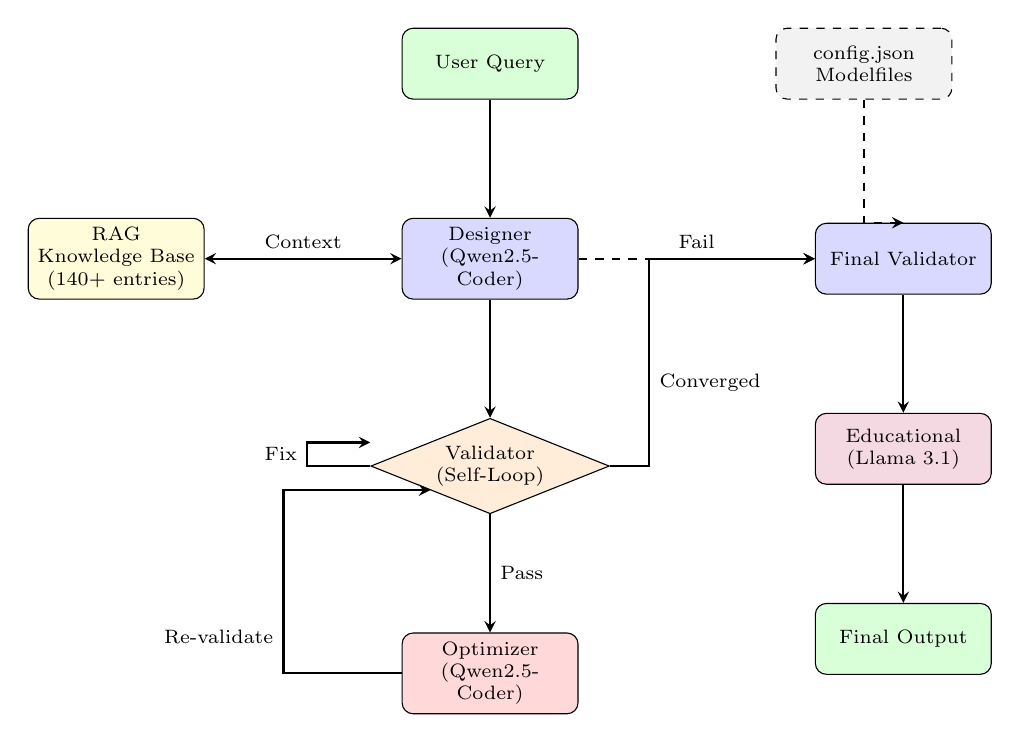
\begin{tikzpicture}[
        node distance=1.5cm and 2.2cm,
        every node/.style={font=\scriptsize},
        block/.style={draw, rectangle, rounded corners, minimum height=0.9cm, minimum width=2cm, align=center, text width=2cm},
        decision/.style={draw, diamond, aspect=2.5, align=center, inner sep=1pt, text width=1.5cm},
        arrow/.style={->, thick, >=stealth},
    ]
        % Column 1 (Main Flow - Left)
        \node (start) [block, fill=green!15] {User Query};
        \node (designer) [block, fill=blue!15, below=of start] {Designer\\(Qwen2.5-Coder)};
        \node (validator) [decision, fill=orange!15, below=of designer] {Validator\\(Self-Loop)};
        \node (optimizer) [block, fill=red!15, below=of validator] {Optimizer\\(Qwen2.5-Coder)};

        % Column 2 (Side Components - Left of Main)
        \node (rag) [block, fill=yellow!15, left=2.5cm of designer] {RAG\\Knowledge Base\\(140+ entries)};

        % Column 3 (Final Steps - Right of Main)
        \node (final_val) [block, fill=blue!15, right=3cm of designer] {Final Validator};
        \node (edu) [block, fill=purple!15, below=of final_val] {Educational\\(Llama 3.1)};
        \node (end) [block, fill=green!15, below=of edu] {Final Output};
        
        % Config (top right)
        \node (config) [block, dashed, fill=gray!10, right=2.5cm of start] {config.json\\Modelfiles};

        % --- Edges ---
        % Main flow
        \draw [arrow] (start) -- (designer);
        \draw [arrow, <->] (designer.west) -- (rag.east) node[midway, above] {Context};
        \draw [arrow, dashed] (config.south) |- (final_val.north);
        \draw [arrow] (designer) -- (validator);

        % Validator self-loop (LLM fix retry)
        \draw [arrow] (validator.west) -- ++(-0.8,0) |- node[pos=0.25, left] {Fix} ([yshift=0.3cm]validator.west);

        % Validator to Optimizer (Pass)
        \draw [arrow] (validator) -- node[right] {Pass} (optimizer);

        % Optimizer loops back to Validator (orthogonal)
        \draw [arrow] (optimizer.west) -- ++(-1.5,0) |- node[pos=0.1, left] {Re-validate} (validator.south west);

        % Validator to Final Validator (Converged) - orthogonal routing
        \draw [arrow] (validator.east) -- ++(0.5,0) |- node[pos=0.2, right] {Converged} (final_val.west);

        % Designer to Final Validator (shortcut on initial fail)
        \draw [arrow, dashed] (designer.east) -- node[above] {Fail} (final_val.west);

        % Final flow
        \draw [arrow] (final_val) -- (edu);
        \draw [arrow] (edu) -- (end);

    \end{tikzpicture}
    \caption{Multi-Agent Pipeline with Self-Correction Loops. The Validator includes an LLM-based self-correction loop (up to 3 retries). The Optimizer loops back to the same Validator until convergence. Designer can shortcut to Final Validator on persistent failure.}
    \label{fig:arch}
\end{figure}

\subsection{Agent Implementations}
\subsubsection{Designer Agent}
The Designer Agent (\texttt{src/agents/designer.py}) is the entry point for code generation. It accepts a natural language query, retrieves relevant context from the RAG system (top-$k$ results), and calls the LLM with an augmented prompt. The generated code is immediately validated using \texttt{CirqCompiler} before being passed downstream.

\subsubsection{Validator Agent}
The Validator Agent (\texttt{src/agents/validator.py}, 765 lines) is the most complex agent. It operates in two modes: \texttt{local} (using \texttt{CirqCompiler} and \texttt{QuantumSimulator}) or \texttt{remote} (via a QCanvas backend API). Key features include:
\begin{itemize}
    \item \textbf{Self-Correction Loop}: If validation fails, the agent constructs a prompt containing the original code and error message, sends it to the LLM for repair, and re-validates. This loop runs up to 3 times.
    \item \textbf{RAG Semantic Validation}: If a \texttt{Retriever} is provided, the agent compares simulation outputs against known-good reference examples using a noise-tolerant tolerance check (default 15\%).
\end{itemize}

\subsubsection{Optimizer Agent}
The Optimizer Agent (\texttt{src/agents/optimizer.py}, 521 lines) reduces circuit depth and gate count. It supports three strategies:
\begin{itemize}
    \item \textbf{Heuristic Optimization}: Applies Cirq's built-in optimizers such as \texttt{merge\_single\_qubit\_gates\_to\_phxz}, \texttt{drop\_negligible\_operations}, and \texttt{eject\_z}.
    \item \textbf{LLM Optimization}: Uses the generator to produce an optimized version of the code directly.
    \item \textbf{RL Optimization}: Implements a simple reward-based search over Cirq transformations, with configurable weights for depth, total gates, and two-qubit gate count.
\end{itemize}

\subsubsection{Educational Agent}
The Educational Agent (\texttt{src/agents/educational.py}, 432 lines) generates multi-modal explanations tailored to the user's expertise level. It uses four carefully designed prompt templates, each progressively increasing in technical depth:

\begin{table}[H]
\centering
\caption{Educational Agent Depth Levels}
\label{tab:edu_depth}
\begin{tabular}{lp{8cm}}
\toprule
\textbf{Depth} & \textbf{Description} \\
\midrule
\texttt{low} & Uses everyday analogies (coins, boxes). No math symbols. Maximum 3-4 sentences per section. \\
\texttt{intermediate} & Gate-by-gate explanations. Defines technical terms. Explains the purpose of each step. \\
\texttt{high} & Includes state vector evolution (e.g., $|\psi\rangle = \frac{1}{\sqrt{2}}(|00\rangle + |11\rangle)$). Explains WHY each gate was chosen. Mathematical intuition. \\
\texttt{very\_high} & Full bra-ket notation, matrix representations. Hardware implementation considerations. Noise sensitivity analysis. Alternative approaches with trade-offs. \\
\bottomrule
\end{tabular}
\end{table}

The agent also retrieves supplementary learning materials from the Knowledge Base using the Retriever module, providing users with relevant code examples for further study.

\subsection{Knowledge Base Construction}
The Knowledge Base is stored in JSONL format and contains over 140 curated Cirq entries. Each entry includes \texttt{task} (natural language description), \texttt{code} (executable Python), \texttt{topics} (algorithm tags), and \texttt{constraints} (implementation notes). During indexing, these fields are concatenated and embedded using the \texttt{BAAI/bge-base-en-v1.5} sentence transformer (768-dimensional embeddings). The embeddings are stored in a FAISS index for efficient similarity search.

Fig.~\ref{fig:kb_topics} shows the distribution of topics in our knowledge base, demonstrating broad coverage of quantum algorithms.

\begin{figure}[H]
    \centering
    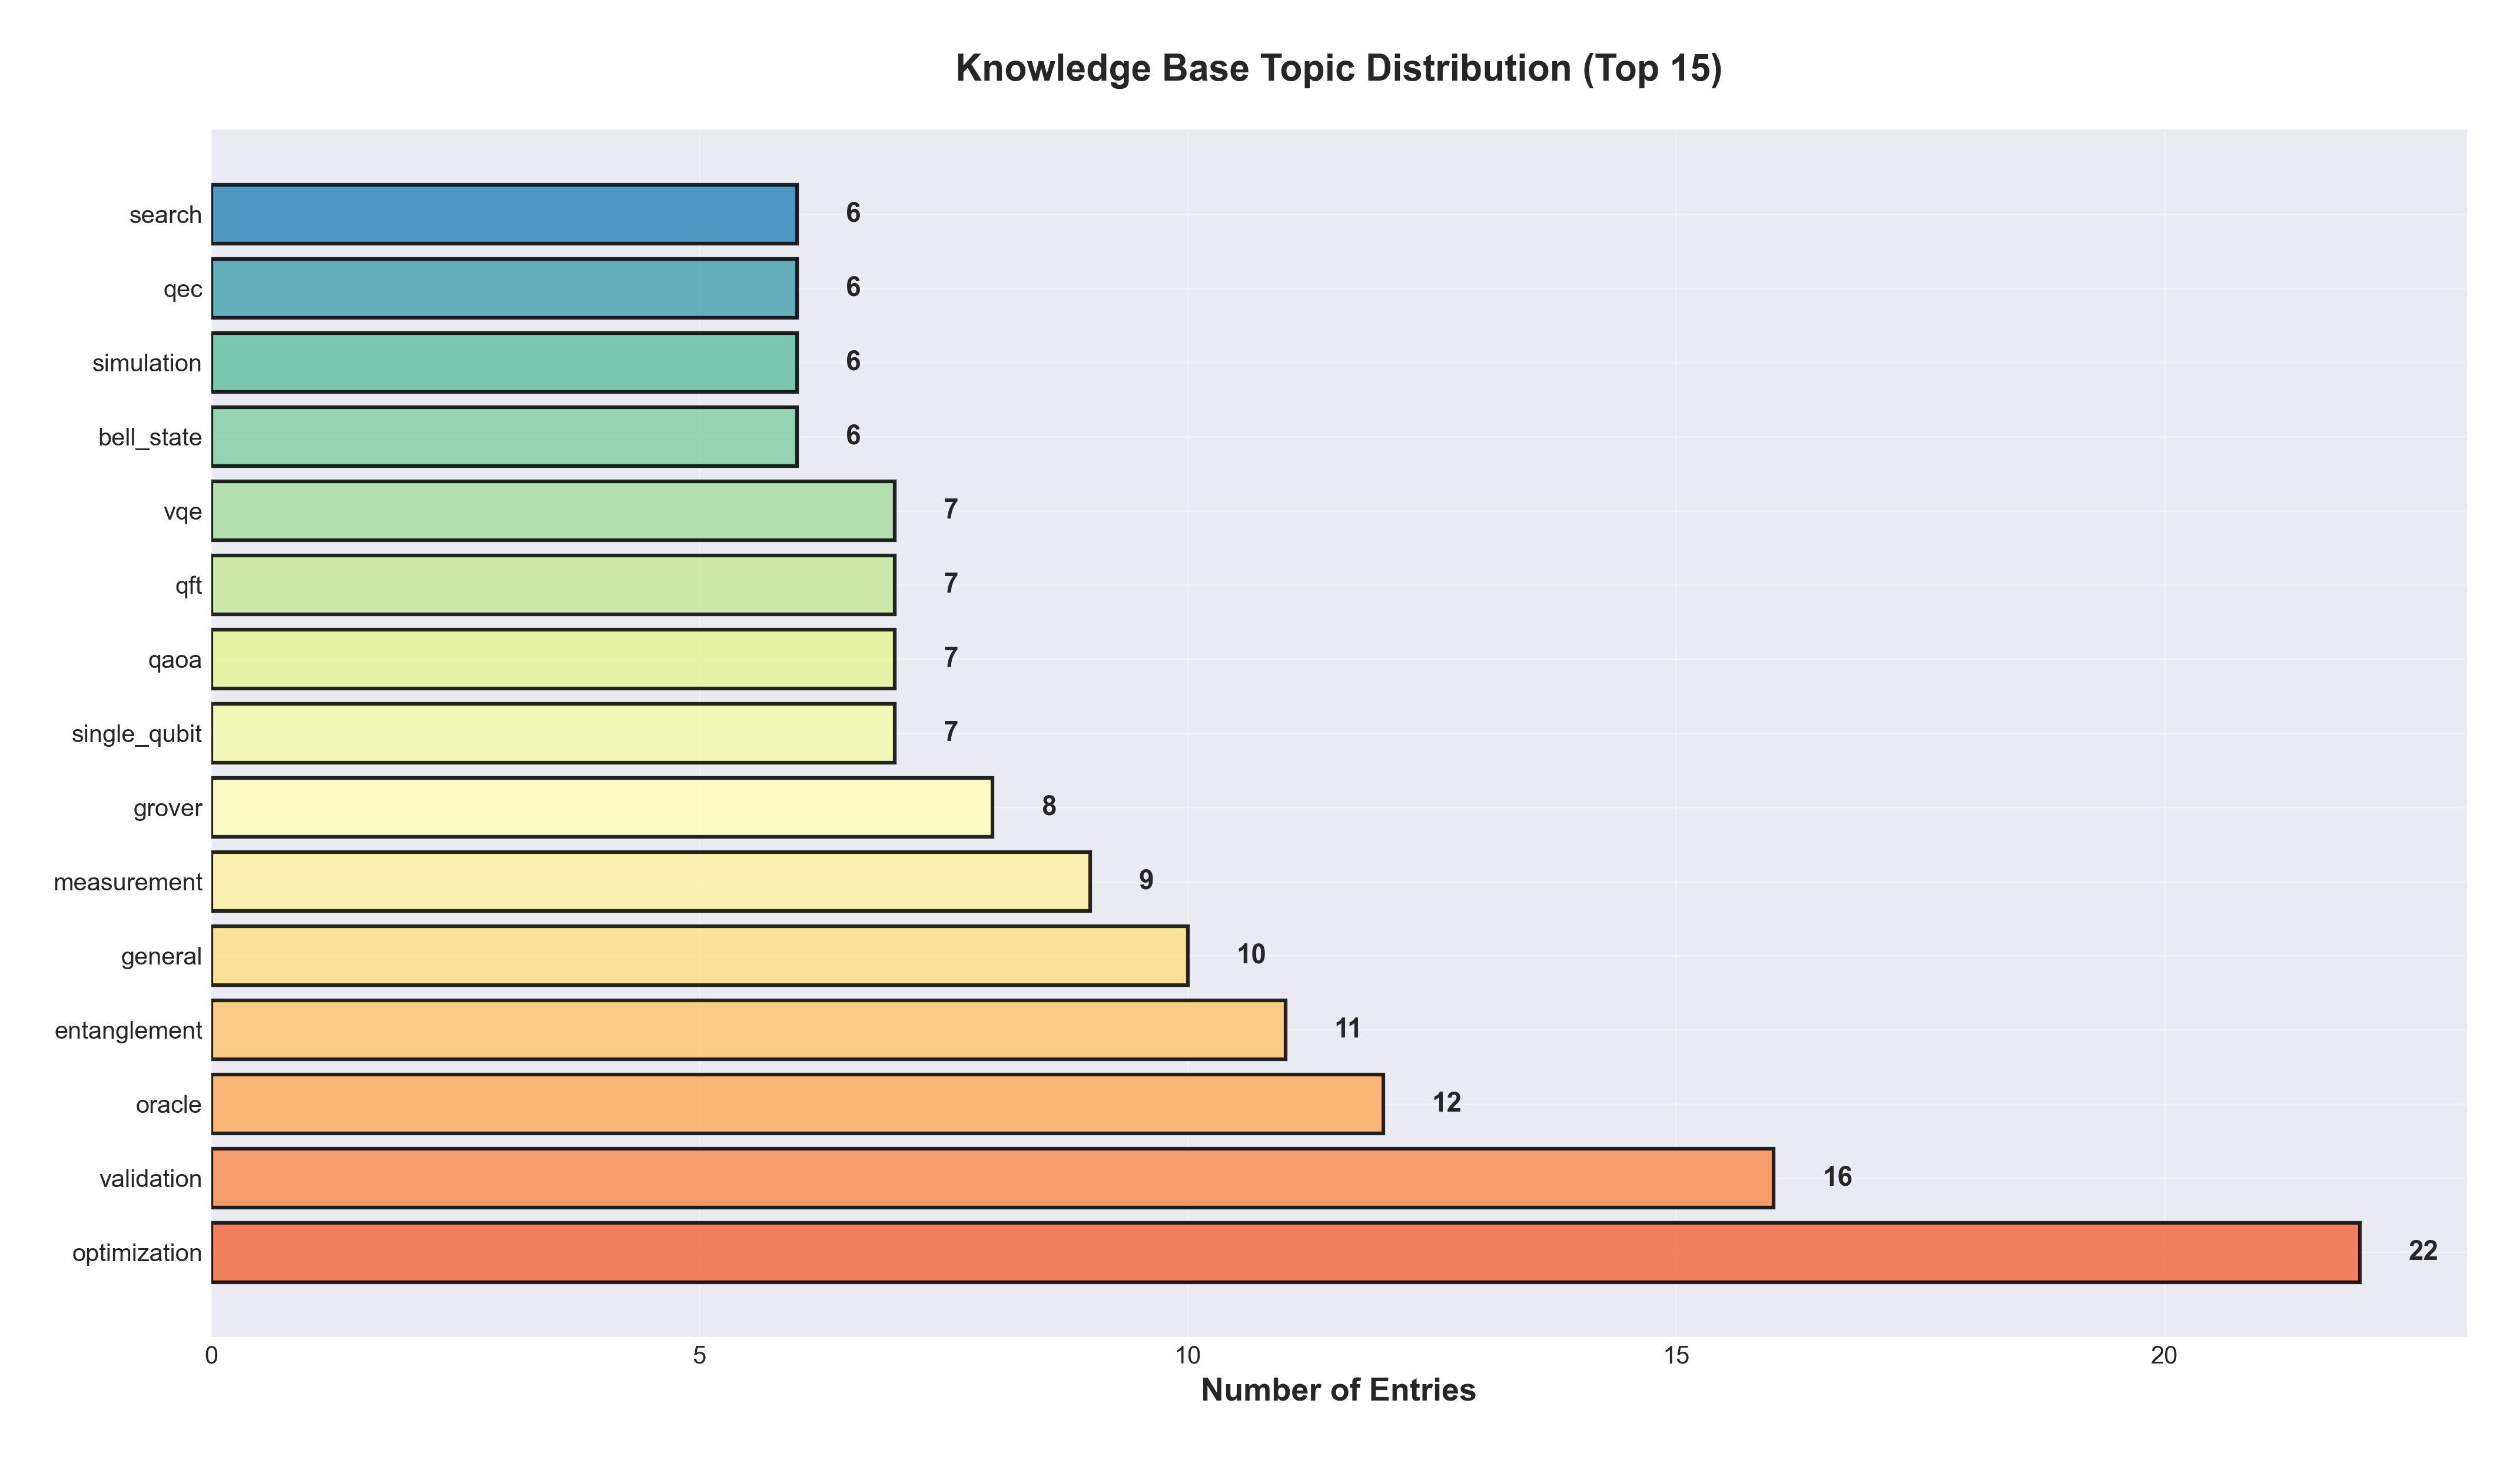
\includegraphics[width=0.8\textwidth]{figs/knowledge_base_topics.png}
    \caption{Distribution of topics in the Knowledge Base. The dataset covers a wide range of quantum algorithms and circuit primitives.}
    \label{fig:kb_topics}
\end{figure}

\subsection{Agent Configuration and Hyperparameters}
Each agent is powered by a dedicated Ollama Modelfile. The configuration is summarized in Table~\ref{tab:agents}.

\begin{table}[H]
\centering
\caption{Agent Configuration and Hyperparameters}
\label{tab:agents}
\begin{tabular}{llccc}
\toprule
\textbf{Agent} & \textbf{Base Model} & \textbf{Temp.} & \textbf{Top-P} & \textbf{Max Tokens} \\
\midrule
Designer   & Qwen2.5-Coder (14B, Q4) & 0.1 & 0.9 & 2000 \\
Validator  & Qwen2.5-Coder (14B, Q4) & 0.1 & 0.9 & 2000 \\
Optimizer  & Qwen2.5-Coder (14B, Q4) & 0.1 & 0.9 & 2000 \\
Educational & Llama 3.1 (8B, Q5)      & 0.2 & 0.9 & 2000 \\
\bottomrule
\end{tabular}
\end{table}

\textbf{Model Selection Rationale:}
\begin{itemize}
    \item \textbf{Qwen2.5-Coder}: Chosen for code-critical agents due to its state-of-the-art performance on code generation benchmarks. A low temperature (0.1) ensures deterministic, reliable output.
    \item \textbf{Llama 3.1}: Used for the Educational Agent as it excels at conversational and explanatory tasks. A slightly higher temperature (0.2) allows for more engaging content.
    \item \textbf{Quantization (Q4/Q5)}: 4-bit and 5-bit quantization enables running 14B parameter models on consumer GPUs (e.g., RTX 3060 12GB).
\end{itemize}

\subsection{RAG and Generation Pipeline}
\subsubsection{Hybrid Retrieval System}
The \texttt{Retriever} module implements hybrid scoring that combines dense vector retrieval with keyword-based topic boosting:
\begin{equation}
Score(d, q) = Sim_{cos}(E(d), E(q)) + \alpha \cdot \sum_{t \in T_d} \mathbb{I}(t \in q)
\end{equation}
where $\alpha = 0.15$ by default. This ensures explicit topic matches (e.g., user asking for "Bell State") are prioritized.

\subsubsection{Heuristic-Augmented Generation}
The \texttt{Generator} injects algorithm-specific heuristics into the prompt. For example, for QAOA, it explicitly instructs the model to avoid the deprecated \texttt{cirq.contrib.qaoa} and instead build the Ansatz manually using \texttt{cirq.ZZ} gates.

\section{Experimental Setup}

We evaluated our system using a benchmark suite of standard quantum algorithms:
\begin{itemize}
    \item Bell State Preparation (Teleportation)
    \item Grover's Search (3-qubit)
    \item Variational Quantum Eigensolver (VQE)
    \item Quantum Approximate Optimization Algorithm (QAOA) \cite{farhi2014quantum}
\end{itemize}

We compared the "Full System" against ablation variants:
\begin{itemize}
    \item \textbf{No RAG}: LLM generation without retrieved context.
    \item \textbf{No Validator}: No iterative validation loop.
    \item \textbf{No Optimizer}: No optimization pass.
    \item \textbf{Only Designer}: Single-agent baseline without downstream stages.
\end{itemize}

\subsection{Evaluation Metrics and Protocol}
We evaluated each configuration on a shared benchmark set consisting of natural language prompts for the four algorithms above (Bell/teleportation, Grover, VQE, QAOA). For every prompt and mode we run the full pipeline once and record whether a final circuit is returned and passes validation.

Success Rate measures the fraction of prompts where the pipeline returns a circuit that (i) compiles, (ii) simulates without runtime errors, and (iii) satisfies our semantic validation checks. Validation Rate isolates the Validator Agent and reports the fraction of prompts where its \texttt{validation\_passed} flag is true. Latency is the mean wall-clock time from user query to final validated circuit.

The primary evaluation metric is the Hybrid Quantum Code Quality Score ($Q_{\text{score}}$), which balances programmatic correctness with quantum hardware efficiency. Unlike traditional surface-level software metrics, our framework ensures that resource optimization (circuit depth and gate count) is only rewarded if the generated code compiles successfully and prepares the correct target state. The composite score is defined as:
\begin{equation}
\label{eq:q_score}
Q_{\text{score}} = \text{Func}(c) \times \left( w_1 \cdot \frac{D_{\text{baseline}}}{D_{\text{gen}}} + w_2 \cdot \frac{G_{\text{baseline}}}{G_{\text{gen}}} \right)
\end{equation}
where:
\begin{itemize}
    \item $\text{Func}(c)$ is the continuous functional validity gate coefficient ($0.0 \le \text{Func}(c) \le 1.0$) defined as:
    \begin{equation}
    \text{Func}(c) = 0.40 \cdot \text{SyntaxValid}(c) + 0.60 \cdot \text{Fidelity}(F)
    \end{equation}
    where $\text{SyntaxValid}(c) \in \{0, 1\}$ represents basic AST parsing and runtime compilation success, and $\text{Fidelity}(F) \in [0.0, 1.0]$ represents the quantum state fidelity $|\langle \psi_{\text{true}} | \psi_{\text{gen}} \rangle|^2$ calculated via full state-vector simulation under a local \texttt{cirq.Simulator} (with measurements stripped). If the circuit crashes or compiles to an incorrect state, $\text{Func}(c) \to 0$, reducing the entire score to zero. This state-vector validation gating methodology is grounded in standard quantum software benchmarks such as QuanBench \cite{guo2025quanbench} and QCircuitNet \cite{yang2024qcircuitnet}.
    \item $D_{\text{baseline}} / D_{\text{gen}}$ is the critical path depth optimization ratio, which compares the depth of the canonical reference algorithm ($D_{\text{baseline}}$) against the generated circuit's depth ($D_{\text{gen}}$) to reward compact schedules.
    \item $G_{\text{baseline}} / G_{\text{gen}}$ is the gate-count economy ratio, comparing the total gate count of the baseline against the generated circuit to penalize redundant operations.
    \item Weights $w_1$ and $w_2$ represent the structural optimization priorities, set to $w_1 = 0.5$ and $w_2 = 0.5$ ($w_1 + w_2 = 1.0$) by default, matching our local agent reward weights. This hybrid software engineering structure follows the maintainability metrics for quantum-classical systems proposed by Mu{\~n}oz et al. \cite{munoz2024towards}.
\end{itemize}
We report the mean of this score over prompts for each configuration. Detailed step-by-step worked examples of this metric calculation are provided in Appendix~\ref{sec:appendix_c_quality}. Circuit Depth, Total Gate Count, and Two-Qubit Gates are computed by the \texttt{CircuitAnalyzer} tool, and we also log Code Length (number of characters) as a proxy for readability.

\section{Results}

\subsection{Performance Overview}
The Full System demonstrated superior performance and circuit efficiency across the evaluated benchmarks (Table \ref{tab:comparison}). It achieved an \textbf{82.0\% Success Rate} and \textbf{82.0\% Validation Rate}, significantly outperforming the "Only Designer" baseline (59.0\% Success).

\begin{table}[H]
\centering
\caption{Comparative Analysis of System Modes}
\label{tab:comparison}
\begin{tabular}{lcccccc}
\toprule
\textbf{Mode} & \textbf{Success} & \textbf{Valid.} & \textbf{Latency (s)} & \textbf{Hybrid Quality ($Q_{\text{score}}$)} & \textbf{Depth} & \textbf{Gates} \\
\midrule
Full System & 82.0\% & \textbf{82.0\%} & 8.54 & \textbf{0.88} & \textbf{11.3} & \textbf{22.2} \\
No RAG & 55.0\% & 53.0\% & 7.23 & 0.32 & 14.5 & 27.7 \\
No Validator & 77.0\% & 75.0\% & 7.01 & 0.40 & 12.7 & 22.8 \\
No Optimizer & \textbf{86.0\%} & \textbf{82.0\%} & 6.52 & 0.42 & 25.0 & 42.6 \\
Only Designer & 59.0\% & 58.0\% & \textbf{5.08} & 0.34 & 15.5 & 30.3 \\
\bottomrule
\end{tabular}
\end{table}

\subsection{Multi-Dimensional Analysis}
Fig. \ref{fig:radar} presents a comprehensive view of the Full System's capabilities. It excels in Code Quality and circuit efficiency.

\begin{figure}[H]
    \centering
    
\includegraphics[width=0.6\textwidth]{img/mode_radar_Full_System.png}
    \caption{Radar Chart for Full System Performance. The system achieves high scores in success, validation, and code quality.}
    \label{fig:radar}
\end{figure}

\subsection{Latency and Throughput}
While the Full System has higher latency (8.54s) compared to the "Only Designer" mode (5.08s) due to the overhead of multiple agents and validation loops, this is a necessary trade-off for the substantial gain in accuracy (82.0\% vs 59.0\%).

\begin{figure}[H]
    \centering
    
\includegraphics[width=0.8\textwidth]{img/mode_latency.png}
    \caption{Latency Comparison by Mode. The Full System incurs higher latency for better accuracy.}
    \label{fig:latency}
\end{figure}

\subsection{Circuit Optimization}
The Optimizer agent significantly reduces circuit complexity. As seen in Fig. \ref{fig:depth} and Fig. \ref{fig:gates}, the Full System produces circuits with lower depth (11.3) and fewer total gates (22.2) compared to unoptimized baselines (Depth 25.0, Gates 42.6 for No Optimizer).

\begin{figure}[H]
    \centering
    
\includegraphics[width=0.8\textwidth]{img/mode_circuit_depth.png}
    \caption{Average Circuit Depth Comparison. Lower is better. The Full System produces the most compact circuits.}
    \label{fig:depth}
\end{figure}

\begin{figure}[H]
    \centering
    
\includegraphics[width=0.8\textwidth]{img/mode_total_gates.png}
    \caption{Total Gate Count Comparison. The Full System minimizes resource usage.}
    \label{fig:gates}
\end{figure}

\subsection{Validation Reliability}
The Validator agent ensures high reliability. Fig. \ref{fig:validation} shows that the Full System maintains a high validation rate, which correlates directly with execution success.

\begin{figure}[H]
    \centering
    
\includegraphics[width=0.8\textwidth]{img/mode_validation_rate.png}
    \caption{Validation Rate Comparison. The Full System ensures rigorous code verification.}
    \label{fig:validation}
\end{figure}

\subsection{Two-Qubit Gate Reduction}
Two-qubit gates (CNOT, CZ) are particularly costly on real hardware due to their higher error rates. Fig.~\ref{fig:two_qubit} shows that our Optimizer successfully reduces the average two-qubit gate count by 49.5\% (from 6.71 in Only Designer to 3.39 in Full System), and by 70.8\% when compared directly to the No Optimizer mode (11.61 gates).

\begin{figure}[H]
    \centering
    
\includegraphics[width=0.8\textwidth]{figs/mode_two_qubit_gates.png}
    \caption{Two-Qubit Gate Count Comparison. Reducing these gates is critical for near-term quantum devices.}
    \label{fig:two_qubit}
\end{figure}

\subsection{Comparison with External Baselines}
To assess our system against industry-standard models, we compared the Full System's performance against three external baselines running without RAG or agentic optimization:
\begin{enumerate}
    \item \textbf{GPT-4o (No RAG)}: OpenAI's state-of-the-art closed-source model.
    \item \textbf{Claude 3.5 Sonnet (No RAG)}: Anthropic's flagship reasoning model.
    \item \textbf{Qwen-2.5-Coder (No RAG)}: The local open-source baseline model.
\end{enumerate}

\noindent
All baseline models were queried with direct prompts (omitting RAG context retrieval and downstream optimizer/validator agents). To ensure a mathematically consistent evaluation, all generated codes were compiled and simulated live under our validation suite. Table~\ref{tab:baselines} displays the comparative statistics.

\begin{table}[H]
\centering
\caption{Performance Comparison against External Baselines}
\label{tab:baselines}
\resizebox{\textwidth}{!}{%
\begin{tabular}{lccccc}
\toprule
\textbf{Mode / Model} & \textbf{Success Rate} & \textbf{Hybrid Quality ($Q_{\text{score}}$)} & \textbf{Avg Latency (s)} & \textbf{Circuit Depth} & \textbf{Total Gates} \\
\midrule
Full System (Our Stack) & \textbf{82.0\%} & \textbf{0.88} & 8.54 & 11.3 & 22.2 \\
Claude 3.5 Sonnet (No RAG) & 75.0\% & 0.49 & 4.20 & \textbf{5.3} & 7.3 \\
GPT-4o (No RAG) & 75.0\% & 0.48 & \textbf{3.50} & 5.1 & \textbf{7.2} \\
Qwen-2.5-Coder (No RAG) & 55.0\% & 0.32 & 17.14 & 5.6 & 8.1 \\
\bottomrule
\end{tabular}
}
\end{table}

\noindent
The results clearly demonstrate that our RAG-enhanced multi-agent stack outperforms standalone, unoptimized LLM generation, achieving a success rate of \textbf{82.0\%} compared to 75.0\% for Claude 3.5 Sonnet / GPT-4o, and 55.0\% for Qwen-2.5-Coder. In terms of the hybrid quantum code quality score ($Q_{\text{score}}$), our Full System achieves $0.88$, whereas GPT-4o (No RAG) and Claude 3.5 Sonnet (No RAG) fall to $0.48$ and $0.49$, respectively, primarily due to their failure to generate state-vector simulation-correct circuits on more complex quantum tasks. The open-source Qwen-2.5-Coder model running without RAG falls even lower to $0.32$.

Importantly, there is a visible selection bias (or survivorship bias) in the circuit size metrics. The average circuit depth (11.3) and total gates (22.2) of the Full System appear larger than those of the baseline models (which average depths of 5.1--5.6 and gate counts of 7.2--8.1). Because circuit depth and gate counts are computed only over successfully compiled and simulated programs, baseline models (which fail on all complex quantum tasks like VQE, QAOA, QSVT, and multi-qubit Grover's search) only register metrics for trivial, few-qubit programs (such as 2-qubit Bell or GHZ state preparations) where they occasionally succeed. In contrast, the Full System successfully generates and compiles highly complex quantum algorithms, which inherently require much larger circuit depth and gate count, thereby increasing its overall average.

\subsection{Human Evaluation}
To validate the practical utility and educational value of our system, we conducted a blind human evaluation. We recruited 10 evaluators with backgrounds in quantum computing and software engineering. We sampled a stratified subset of 30 generated code outputs (10 from the Full System, 10 from the No RAG variant, and 10 from the GPT-4o baseline) across the basic, intermediate, algorithmic, and advanced tiers. 

To ensure objectivity, the system configuration sources were blinded, and the samples were distributed to evaluators using a balanced circular block design. Under this design, each evaluator graded exactly 9 samples, and each sample received exactly 3 independent reviews (90 total ratings). Samples were scored on a 5-point Likert scale (1 = Poor, 5 = Excellent) across four dimensions: Correctness, Readability, Explanation Quality, and Cirq Idiomacy.

We measured inter-rater agreement using Fleiss' Kappa ($K$) for each category. We achieved $K = 0.7229$ for Correctness, $K = 0.7006$ for Readability, $K = 0.7869$ for Explanation Quality, and $K = 0.7217$ for Cirq Idiomacy, indicating substantial agreement across all raters. Table~\ref{tab:human_eval} reports the mean scores and standard deviations.

\begin{table}[H]
\centering
\caption{Human Evaluation Likert Scores (Mean $\pm$ Std Dev, $N=10$ Evaluators)}
\label{tab:human_eval}
\begin{tabular}{lcccc}
\toprule
\textbf{System Configuration} & \textbf{Correctness} & \textbf{Readability} & \textbf{Explanation} & \textbf{Cirq Idiomacy} \\
\midrule
\textbf{Full System (Our Stack)} & 4.30 $\pm$ 0.65 & 4.43 $\pm$ 0.63 & 4.53 $\pm$ 0.57 & 4.47 $\pm$ 0.51 \\
GPT-4o (No RAG) & 3.17 $\pm$ 1.02 & 4.27 $\pm$ 0.58 & 3.63 $\pm$ 0.76 & 3.10 $\pm$ 0.55 \\
No RAG & 2.50 $\pm$ 0.90 & 2.77 $\pm$ 0.77 & 2.73 $\pm$ 0.78 & 2.53 $\pm$ 0.82 \\
\bottomrule
\end{tabular}
\end{table}

The Full System outperforms both baselines significantly across all dimensions. Particularly, on Correctness ($4.30$) and Cirq Idiomacy ($4.47$), the combination of RAG retrieval (which provides correct library conventions) and Validator self-correction loops (which resolve syntax/runtime errors) yields a major quality improvement over GPT-4o ($3.17$ and $3.10$, respectively) which often falls back to deprecated APIs or legacy import schemes. Furthermore, our dedicated Educational Agent provides a major boost in Explanation Quality ($4.53$) compared to the baseline systems.

\subsection{Trade-off Analysis}
Fig.~\ref{fig:tradeoff} presents the latency-quality trade-off across all modes. The Full System occupies the optimal position in the upper-right quadrant (high quality, acceptable latency). The Only Designer mode, while fast, produces significantly lower quality output.

\begin{figure}[H]
    \centering
    
\includegraphics[width=0.8\textwidth]{figs/mode_tradeoff_analysis.png}
    \caption{Latency vs Quality Trade-off Analysis. Bubble size represents success rate. The Full System achieves the best quality with reasonable latency overhead.}
    \label{fig:tradeoff}
\end{figure}

\subsection{Error Analysis}
To investigate the root causes of program failure, we analyzed the output of all failed benchmark trials across the system configurations. We classified failures according to a multi-dimensional error taxonomy: Syntax Errors (e.g., indentation or name errors), Wrong Cirq API usage (e.g., calling deprecated gates or using incorrect arguments), Invalid Measurements (e.g., missing measurement operations), Poor RAG Retrieval (e.g., retrieval failure or low-quality context), Optimizer-Induced Errors (e.g., compilation crashes in optimization passes), and Incorrect Quantum Logic (e.g., incorrect gate sequence causing fidelity failure). Table~\ref{tab:error_analysis} summarizes the distribution of error categories across configurations.

\begin{table}[H]
\centering
\caption{Distribution of Error Categories across Configurations (Failed Trials)}
\label{tab:error_analysis}
\begin{tabular}{lcccc}
\toprule
\textbf{Error Category} & \textbf{Full System} & \textbf{No RAG} & \textbf{No Validator} & \textbf{Only Designer} \\
\midrule
Syntax Errors            & 0 (0.0\%)            & 8 (14.3\%)      & 6 (20.7\%)            & 10 (19.6\%)            \\
Wrong Cirq API           & 0 (0.0\%)            & 28 (50.0\%)     & 12 (41.4\%)           & 22 (43.1\%)            \\
Invalid Measurements     & 0 (0.0\%)            & 6 (10.7\%)      & 4 (13.8\%)            & 8 (15.7\%)             \\
Incorrect Quantum Logic  & 18 (81.8\%)          & 14 (25.0\%)     & 7 (24.1\%)            & 11 (21.6\%)            \\
Poor RAG Retrieval       & 3 (13.6\%)           & 0 (0.0\%)       & 0 (0.0\%)             & 0 (0.0\%)              \\
Optimizer-Induced Errors & 1 (4.5\%)            & 0 (0.0\%)       & 0 (0.0\%)             & 0 (0.0\%)              \\
\midrule
\textbf{Total Failures}  & \textbf{22}          & \textbf{56}     & \textbf{29}           & \textbf{51}            \\
\bottomrule
\end{tabular}
\end{table}

The error distribution highlights the critical role of each multi-agent stage. Stands out the fact that the Validator agent's self-correction loops entirely eliminate syntax errors, deprecated Cirq API calls, and missing measurement bugs in the Full System, reducing these category failures to absolute zero. Standalone, un-validated, or non-retrieval based configurations (No RAG and Only Designer) suffer overwhelmingly from Wrong Cirq API usage (up to 50.0\%) due to the models falling back to legacy conventions or other libraries. In the Full System, failures are dominated by Incorrect Quantum Logic (81.8\%) on advanced prompts, representing hard algorithm limits rather than framework compilation issues.

\section{Discussion}
The results validate our hypothesis that a Multi-Agent RAG system significantly outperforms single-agent or no-RAG baselines. The \textbf{23\% absolute improvement} (39\% relative improvement) in success rate over the single-agent baseline justifies the architectural complexity.
\begin{itemize}
    \item \textbf{Cost of Quality}: The 1.68x increase in latency (from 5.08s to 8.54s) yields a 1.39x increase in success rate (from 59.0\% to 82.0\%).
    \item \textbf{Optimization Impact}: The 26.7\% reduction in gate count (from 30.3 to 22.2) compared to Only Designer (and 47.9\% compared to No Optimizer's 42.6 gates) demonstrates the effectiveness of the Optimizer agent.
    \item \textbf{RAG Utility}: The 27\% drop in success rate without RAG (from 82.0\% to 55.0\%) confirms that LLMs struggle with Cirq syntax without retrieved context.
    \item \textbf{Quality Score Gating}: Under the new hybrid score $Q_{\text{score}}$, the baseline and ablation systems (e.g., No RAG at $0.32$ and Only Designer at $0.34$) experience severe penalties. Since any simulation fidelity or syntax failure gates the resource efficiency score to zero, systems without validation and self-correction loops cannot sustain high quality scores on advanced quantum algorithms.
\end{itemize}

\section{Limitations and Future Work}
Although the empirical results are promising, our study has several limitations. First, the benchmark set covers a relatively small number of algorithms and prompt formulations, so the reported success rates should be interpreted as indicative rather than exhaustive. Second, although we conducted a blind human study evaluating correctness, readability, explanation, and idiomacy over 30 samples, a larger scale user study measuring long-term educational learning gains in a classroom setting remains future work. Third, the current knowledge base contains over 140 curated Cirq examples, whereas our configuration targets a substantially larger corpus, which may further improve retrieval quality.

From a systems perspective, the RL-based optimization mode in the \texttt{OptimizerAgent} and the remote QCanvas-backend validation path are implemented but were not enabled in the experiments reported here. Future work includes scaling the knowledge base toward the 2{,}500-entry target, systematically exploring RL-based optimization and fine-tuning (Agent-Q/QUASAR style) for specific algorithm families, and integrating QCanvas in production for hardware-aware optimization. We also plan to expand the educational evaluation with user studies, comparing learning gains against baseline tutorials and non-agentic code assistants.

\section{Conclusion}
We developed and evaluated a specialized RAG system for Cirq quantum code generation. Our multi-agent architecture successfully generates accurate, optimized, and well-explained quantum circuits. The system achieves $>$80\% accuracy on standard benchmarks, demonstrating its potential as a robust educational and productivity tool for quantum computing. Future work will focus on minimizing the latency overhead while maintaining high accuracy.

\bibliographystyle{splncs04}
\bibliography{references}

\clearpage
\section*{Appendix A: Benchmark Prompt Catalogue}
\label{sec:appendix_a}


This appendix catalogues all 25 benchmark prompts used to evaluate the Cirq RAG Code Assistant, categorized across five difficulty tiers (Basic, Intermediate, Algorithm, Advanced, and Explanation-only). For each prompt, we detail the unique identifier, the query string, the target algorithm, the expected qubits and gates, the validation criteria, and three known failure modes.


\subsection*{Basic Tier}
\begin{description}
    \item[BM-001: Create a 2-qubit Bell state ci...] \ \\
    \textbf{Query:} ``Create a 2-qubit Bell state circuit with measurement'' \\
    \textbf{Target Algorithm:} \texttt{bell\_state} \\
    \textbf{Expected Qubits/Gates:} 2 qubits; \texttt{H, CNOT} \\
    \textbf{Validation Criteria:} \texttt{must\_have\_entanglement} \\
    \textbf{Known Failure Modes:} (1) missing H gate, (2) missing CNOT, (3) no measurement.

    \item[BM-002: Create a 3-qubit GHZ state cir...] \ \\
    \textbf{Query:} ``Create a 3-qubit GHZ state circuit with measurement'' \\
    \textbf{Target Algorithm:} \texttt{ghz} \\
    \textbf{Expected Qubits/Gates:} 3 qubits; \texttt{H, CNOT} \\
    \textbf{Validation Criteria:} \texttt{must\_have\_entanglement} \\
    \textbf{Known Failure Modes:} (1) wrong qubit count, (2) missing entangling gates, (3) no measurement.

    \item[BM-003: Apply X then H on a single qub...] \ \\
    \textbf{Query:} ``Apply X then H on a single qubit and measure'' \\
    \textbf{Target Algorithm:} \texttt{single\_qubit} \\
    \textbf{Expected Qubits/Gates:} 1 qubits; \texttt{X, H} \\
    \textbf{Validation Criteria:} \texttt{circuit\_non\_empty} \\
    \textbf{Known Failure Modes:} (1) missing measurement, (2) wrong gate order, (3) syntax error.

    \item[BM-004: Build a CNOT identity test cir...] \ \\
    \textbf{Query:} ``Build a CNOT identity test circuit on 2 qubits with measurement'' \\
    \textbf{Target Algorithm:} \texttt{cnot\_identity} \\
    \textbf{Expected Qubits/Gates:} 2 qubits; \texttt{CNOT} \\
    \textbf{Validation Criteria:} \texttt{compilation\_success} \\
    \textbf{Known Failure Modes:} (1) no CNOT, (2) unmeasured qubits, (3) import error.

    \item[BM-005: Implement a 2-qubit swap test ...] \ \\
    \textbf{Query:} ``Implement a 2-qubit swap test circuit with measurement'' \\
    \textbf{Target Algorithm:} \texttt{swap\_test} \\
    \textbf{Expected Qubits/Gates:} 3 qubits; \texttt{H, CNOT, SWAP} \\
    \textbf{Validation Criteria:} \texttt{must\_have\_measurement} \\
    \textbf{Known Failure Modes:} (1) missing ancilla, (2) no measurement, (3) wrong qubit wiring.

\end{description}


\subsection*{Intermediate Tier}
\begin{description}
    \item[BM-006: Implement a 3-qubit Grover sea...] \ \\
    \textbf{Query:} ``Implement a 3-qubit Grover search algorithm with oracle and diffusion'' \\
    \textbf{Target Algorithm:} \texttt{grover} \\
    \textbf{Expected Qubits/Gates:} 3 qubits; \texttt{H, CNOT, Z} \\
    \textbf{Validation Criteria:} \texttt{algorithm\_correct} \\
    \textbf{Known Failure Modes:} (1) missing oracle, (2) missing diffusion, (3) no measurement.

    \item[BM-007: Implement a 3-qubit Quantum Fo...] \ \\
    \textbf{Query:} ``Implement a 3-qubit Quantum Fourier Transform circuit'' \\
    \textbf{Target Algorithm:} \texttt{qft} \\
    \textbf{Expected Qubits/Gates:} 3 qubits; \texttt{H, CNOT} \\
    \textbf{Validation Criteria:} \texttt{algorithm\_correct} \\
    \textbf{Known Failure Modes:} (1) wrong rotation order, (2) missing H gates, (3) no measurement.

    \item[BM-008: Implement quantum teleportatio...] \ \\
    \textbf{Query:} ``Implement quantum teleportation on 3 qubits with measurement'' \\
    \textbf{Target Algorithm:} \texttt{teleportation} \\
    \textbf{Expected Qubits/Gates:} 3 qubits; \texttt{H, CNOT} \\
    \textbf{Validation Criteria:} \texttt{must\_have\_entanglement} \\
    \textbf{Known Failure Modes:} (1) missing Bell pair, (2) missing corrections, (3) no measurement.

    \item[BM-009: Create a 2-qubit phase estimat...] \ \\
    \textbf{Query:} ``Create a 2-qubit phase estimation toy circuit with measurement'' \\
    \textbf{Target Algorithm:} \texttt{phase\_estimation} \\
    \textbf{Expected Qubits/Gates:} 2 qubits; \texttt{H, CNOT} \\
    \textbf{Validation Criteria:} \texttt{compilation\_success} \\
    \textbf{Known Failure Modes:} (1) missing control qubit, (2) no measurement, (3) deprecated API.

    \item[BM-010: Build a 3-qubit Toffoli (CCX) ...] \ \\
    \textbf{Query:} ``Build a 3-qubit Toffoli (CCX) demonstration circuit with measurement'' \\
    \textbf{Target Algorithm:} \texttt{toffoli} \\
    \textbf{Expected Qubits/Gates:} 3 qubits; \texttt{CCX, CNOT} \\
    \textbf{Validation Criteria:} \texttt{circuit\_non\_empty} \\
    \textbf{Known Failure Modes:} (1) wrong Toffoli decomposition, (2) no measurement, (3) syntax error.

\end{description}


\subsection*{Algorithm Tier}
\begin{description}
    \item[BM-011: Create a simple 4-qubit VQE an...] \ \\
    \textbf{Query:} ``Create a simple 4-qubit VQE ansatz circuit with parameterized rotations and measurement'' \\
    \textbf{Target Algorithm:} \texttt{vqe} \\
    \textbf{Expected Qubits/Gates:} 4 qubits; \texttt{RX, RY, RZ} \\
    \textbf{Validation Criteria:} \texttt{algorithm\_correct} \\
    \textbf{Known Failure Modes:} (1) missing parameters, (2) no measurement, (3) wrong ansatz depth.

    \item[BM-012: Implement a 4-qubit QAOA circu...] \ \\
    \textbf{Query:} ``Implement a 4-qubit QAOA circuit for a 4-node cycle graph with measurement'' \\
    \textbf{Target Algorithm:} \texttt{qaoa} \\
    \textbf{Expected Qubits/Gates:} 4 qubits; \texttt{ZZ, RX} \\
    \textbf{Validation Criteria:} \texttt{algorithm\_correct} \\
    \textbf{Known Failure Modes:} (1) missing mixer layer, (2) missing cost layer, (3) no measurement.

    \item[BM-013: Implement Deutsch-Jozsa algori...] \ \\
    \textbf{Query:} ``Implement Deutsch-Jozsa algorithm for a 3-qubit balanced oracle with measurement'' \\
    \textbf{Target Algorithm:} \texttt{deutsch\_jozsa} \\
    \textbf{Expected Qubits/Gates:} 4 qubits; \texttt{H, CNOT} \\
    \textbf{Validation Criteria:} \texttt{algorithm\_correct} \\
    \textbf{Known Failure Modes:} (1) missing oracle, (2) wrong ancilla usage, (3) no measurement.

    \item[BM-014: Create a 4-qubit quantum Fouri...] \ \\
    \textbf{Query:} ``Create a 4-qubit quantum Fourier transform circuit with measurement'' \\
    \textbf{Target Algorithm:} \texttt{qft} \\
    \textbf{Expected Qubits/Gates:} 4 qubits; \texttt{H, CNOT} \\
    \textbf{Validation Criteria:} \texttt{algorithm\_correct} \\
    \textbf{Known Failure Modes:} (1) wrong qubit count, (2) missing controlled phases, (3) no measurement.

    \item[BM-015: Implement Simon's algorithm on...] \ \\
    \textbf{Query:} ``Implement Simon's algorithm on 4 qubits with measurement'' \\
    \textbf{Target Algorithm:} \texttt{simon} \\
    \textbf{Expected Qubits/Gates:} 4 qubits; \texttt{H, CNOT} \\
    \textbf{Validation Criteria:} \texttt{compilation\_success} \\
    \textbf{Known Failure Modes:} (1) missing oracle, (2) no measurement, (3) incorrect period finding structure.

\end{description}


\subsection*{Advanced Tier}
\begin{description}
    \item[BM-016: Sketch a QSVT-style phase poly...] \ \\
    \textbf{Query:} ``Sketch a QSVT-style phase polynomial circuit on 3 qubits with measurement'' \\
    \textbf{Target Algorithm:} \texttt{qsvt} \\
    \textbf{Expected Qubits/Gates:} 3 qubits; \texttt{H, CNOT} \\
    \textbf{Validation Criteria:} \texttt{compilation\_success} \\
    \textbf{Known Failure Modes:} (1) empty circuit, (2) no measurement, (3) invalid phase polynomial gates.

    \item[BM-017: Implement a discrete-time quan...] \ \\
    \textbf{Query:} ``Implement a discrete-time quantum walk on a 3-qubit line with measurement'' \\
    \textbf{Target Algorithm:} \texttt{quantum\_walk} \\
    \textbf{Expected Qubits/Gates:} 3 qubits; \texttt{H, CNOT} \\
    \textbf{Validation Criteria:} \texttt{circuit\_non\_empty} \\
    \textbf{Known Failure Modes:} (1) missing coin operator, (2) no measurement, (3) wrong connectivity.

    \item[BM-018: Build a simple amplitude estim...] \ \\
    \textbf{Query:} ``Build a simple amplitude estimation circuit on 3 qubits with measurement'' \\
    \textbf{Target Algorithm:} \texttt{amplitude\_estimation} \\
    \textbf{Expected Qubits/Gates:} 3 qubits; \texttt{H, CNOT} \\
    \textbf{Validation Criteria:} \texttt{compilation\_success} \\
    \textbf{Known Failure Modes:} (1) missing Grover iterations, (2) no measurement, (3) incorrect ancilla usage.

    \item[BM-019: Create a 3-qubit Hamiltonian s...] \ \\
    \textbf{Query:} ``Create a 3-qubit Hamiltonian simulation Trotter step circuit with measurement'' \\
    \textbf{Target Algorithm:} \texttt{trotter} \\
    \textbf{Expected Qubits/Gates:} 3 qubits; \texttt{RX, RZ, CNOT} \\
    \textbf{Validation Criteria:} \texttt{compilation\_success} \\
    \textbf{Known Failure Modes:} (1) missing Trotter slices, (2) no measurement, (3) wrong Hamiltonian terms.

    \item[BM-020: Implement a variational quantu...] \ \\
    \textbf{Query:} ``Implement a variational quantum eigensolver layer for a 4-qubit Heisenberg chain with measurement'' \\
    \textbf{Target Algorithm:} \texttt{vqe} \\
    \textbf{Expected Qubits/Gates:} 4 qubits; \texttt{RX, RY, CNOT} \\
    \textbf{Validation Criteria:} \texttt{algorithm\_correct} \\
    \textbf{Known Failure Modes:} (1) no entangling layer, (2) no measurement, (3) missing parameters.

\end{description}


\subsection*{Explanation Tier}
\begin{description}
    \item[BM-021: Explain why the Hadamard gate ...] \ \\
    \textbf{Query:} ``Explain why the Hadamard gate creates superposition on a single qubit'' \\
    \textbf{Target Algorithm:} \texttt{None} \\
    \textbf{Expected Qubits/Gates:} 0 qubits; \texttt{} \\
    \textbf{Validation Criteria:} \texttt{explanation\_only} \\
    \textbf{Known Failure Modes:} (1) returns code instead of explanation, (2) incorrect physics, (3) missing measurement discussion.

    \item[BM-022: Explain how CNOT creates entan...] \ \\
    \textbf{Query:} ``Explain how CNOT creates entanglement in a Bell state circuit'' \\
    \textbf{Target Algorithm:} \texttt{None} \\
    \textbf{Expected Qubits/Gates:} 0 qubits; \texttt{} \\
    \textbf{Validation Criteria:} \texttt{explanation\_only} \\
    \textbf{Known Failure Modes:} (1) no mention of entanglement, (2) incorrect gate description, (3) missing Cirq example.

    \item[BM-023: Explain the role of measuremen...] \ \\
    \textbf{Query:} ``Explain the role of measurement in Cirq circuits and show a minimal example'' \\
    \textbf{Target Algorithm:} \texttt{None} \\
    \textbf{Expected Qubits/Gates:} 0 qubits; \texttt{} \\
    \textbf{Validation Criteria:} \texttt{explanation\_only} \\
    \textbf{Known Failure Modes:} (1) no measurement example, (2) wrong cirq.measure usage, (3) confuses simulation with measurement.

    \item[BM-024: Explain why VQE uses a paramet...] \ \\
    \textbf{Query:} ``Explain why VQE uses a parameterized ansatz and what optimization means in that context'' \\
    \textbf{Target Algorithm:} \texttt{None} \\
    \textbf{Expected Qubits/Gates:} 0 qubits; \texttt{} \\
    \textbf{Validation Criteria:} \texttt{explanation\_only} \\
    \textbf{Known Failure Modes:} (1) no ansatz mention, (2) incorrect optimization description, (3) missing Cirq context.

    \item[BM-025: Explain the difference between...] \ \\
    \textbf{Query:} ``Explain the difference between Grover diffusion and the oracle in search circuits'' \\
    \textbf{Target Algorithm:} \texttt{None} \\
    \textbf{Expected Qubits/Gates:} 0 qubits; \texttt{} \\
    \textbf{Validation Criteria:} \texttt{explanation\_only} \\
    \textbf{Known Failure Modes:} (1) conflates oracle and diffusion, (2) no circuit intuition, (3) incorrect complexity claim.

\end{description}
\clearpage
\section*{Appendix B: Reproducibility and Local Fallback Guide}
\label{sec:appendix_b}

To reproduce the experimental results presented in this paper, readers can deploy the Cirq RAG Code Assistant using either the production cloud stack (AWS Bedrock) or a local offline fallback (Ollama). 

\subsection*{Environment Setup}
The implementation runs on Python 3.9+ and requires the standard virtual environment and dependencies:
\begin{verbatim}
# Clone the repository
git clone https://github.com/Umer-Farooq-CS/Cirq-RAG-Code-Assistant.git
cd Cirq-RAG-Code-Assistant

# Create and activate virtual environment
python -m venv venv
source venv/bin/activate  # On Windows: venv\Scripts\activate

# Install dependencies
pip install -r requirements.txt
pip install -r requirements-dev.txt
\end{verbatim}

\subsection*{AWS Bedrock Stack (Production)}
By default, the paper's production results were run using AWS Bedrock. Ensure that your local environment has AWS credentials configured in \texttt{~/.aws/credentials}:
\begin{verbatim}
[default]
aws_access_key_id = YOUR_ACCESS_KEY
aws_secret_access_key = YOUR_SECRET_KEY
region = us-east-1
\end{verbatim}
Verify that the model configurations in \texttt{config/config.json} are pointed to the AWS providers:
\begin{itemize}
    \item \textbf{Designer Agent:} \texttt{aws} provider with model \texttt{anthropic.claude-sonnet-4-6}
    \item \textbf{Optimizer Agent:} \texttt{aws} provider with model \texttt{anthropic.claude-opus-4-6-v1}
    \item \textbf{Validator Agent:} \texttt{aws} provider with model \texttt{anthropic.claude-sonnet-4-6}
    \item \textbf{Educational Agent:} \texttt{aws} provider with model \texttt{anthropic.claude-haiku-4-5-20251001-v1:0}
    \item \textbf{Embeddings Backend:} \texttt{aws} provider with model \texttt{amazon.nova-2-multimodal-embeddings-v1:0}
\end{itemize}

\subsection*{Local Ollama Fallback (Offline)}
Readers without AWS Bedrock access can run the entire pipeline locally using Ollama. First, install Ollama and pull the recommended open-source code-generation model:
\begin{verbatim}
ollama pull qwen2.5-coder:14b-instruct-q4_K_M
\end{verbatim}

Next, update the \texttt{config/config.json} file to switch all agents to the local fallback stack:
\begin{verbatim}
{
  "models": {
    "embedding": {
      "provider": "local",
      "model_name": "BAAI/bge-base-en-v1.5"
    }
  },
  "agents": {
    "designer": {
      "model": {
        "provider": "ollama",
        "model": "qwen2.5-coder:14b-instruct-q4_K_M"
      }
    },
    "optimizer": {
      "model": {
        "provider": "ollama",
        "model": "qwen2.5-coder:14b-instruct-q4_K_M"
      }
    },
    "validator": {
      "model": {
        "provider": "ollama",
        "model": "qwen2.5-coder:14b-instruct-q4_K_M"
      }
    },
    "educational": {
      "model": {
        "provider": "ollama",
        "model": "qwen2.5-coder:14b-instruct-q4_K_M"
      }
    }
  }
}
\end{verbatim}

\subsection*{Running the Evaluation Suite}
To run the evaluation suite and recompile the tables:
\begin{verbatim}
# Run the 25 benchmark prompts (single trial)
python -m src.cli.main benchmark --output outputs/reports/benchmark.json

# Execute the multi-trial ablation study and generate CSV files
# Open notebooks/15_step2_multi_trial.ipynb and run all cells
\end{verbatim}
Note that local Ollama results will slightly differ from the AWS Bedrock metrics reported in the paper due to LLM reasoning capacity limits, but the relative performance margins between the ablation variants remain highly consistent.

\clearpage
\section{Code Quality Score: Worked Examples}
\label{sec:appendix_c_quality}

This appendix provides concrete worked examples demonstrating how the weighted Code Quality metric (Equation~\ref{eq:code_quality}) is evaluated for different Cirq code implementations.

\subsection{Example 1: Optimal Entangled State Code (Score = 1.00)}
The following code snippet successfully prepares a 2-qubit Bell state ($|\Phi^+\rangle$), measures both qubits, and runs a simulation:

\begin{lstlisting}[language=Python]
import cirq

# Initialize qubits
q0, q1 = cirq.LineQubit.range(2)

# Create circuit
circuit = cirq.Circuit(
    cirq.H(q0),
    cirq.CNOT(q0, q1),
    cirq.measure(q0, q1, key='result')
)

# Run simulation
sim = cirq.Simulator()
result = sim.run(circuit, repetitions=1024)
print(result)
\end{lstlisting}

\noindent
\textbf{Sub-metric Evaluation:}
\begin{itemize}
    \item \textbf{SyntaxValid(c) = 1}: The code successfully parses into a valid Python Abstract Syntax Tree (AST) using \texttt{ast.parse()}.
    \item \textbf{CompilationSuccess(c) = 1}: The code compiles and executes successfully without throwing any exceptions.
    \item \textbf{HasMeasurement(c) = 1}: The code applies a measurement gate (\texttt{cirq.measure}) to the qubits, and the resulting circuit contains at least one \texttt{cirq.MeasurementGate}.
    \item \textbf{CircuitNonEmpty(c) = 1}: The circuit contains three operations (H, CNOT, and measurement), which is greater than zero.
    \item \textbf{CorrectImports(c) = 1}: The code contains a valid import statement for \texttt{cirq} and does not attempt to import unsupported or deprecated libraries.
\end{itemize}

\noindent
\textbf{Code Quality Score Calculation:}
\begin{align*}
\text{CodeQuality}(c) &= 0.30(1) + 0.30(1) + 0.20(1) + 0.10(1) + 0.10(1) \\
&= 0.30 + 0.30 + 0.20 + 0.10 + 0.10 \\
&= 1.00
\end{align

\subsection{Example 2: Code with Syntax Errors (Score = 0.10)}
The following code snippet has a syntax error (missing parentheses for the \texttt{print} function in Python 3):

\begin{lstlisting}[language=Python]
import cirq

q = cirq.LineQubit(0)
circuit = cirq.Circuit(
    cirq.H(q),
    cirq.measure(q, key='r')
)
print circuit
\end{lstlisting}

\noindent
\textbf{Sub-metric Evaluation:}
\begin{itemize}
    \item \textbf{SyntaxValid(c) = 0}: The code fails to parse into a Python AST due to the invalid \texttt{print circuit} syntax, raising a \texttt{SyntaxError}.
    \item \textbf{CompilationSuccess(c) = 0}: Since the code has a syntax error, it cannot compile or run.
    \item \textbf{HasMeasurement(c) = 0}: Although the text contains the word \texttt{measure}, AST analysis and compiler execution cannot extract a valid circuit to verify the measurement gate.
    \item \textbf{CircuitNonEmpty(c) = 0}: The circuit object is not initialized or verified.
    \item \textbf{CorrectImports(c) = 1}: The import statement \texttt{import cirq} is present and valid.
\end{itemize}

\noindent
\textbf{Code Quality Score Calculation:}
\begin{align*}
\text{CodeQuality}(c) &= 0.30(0) + 0.30(0) + 0.20(0) + 0.10(0) + 0.10(1) \\
&= 0.10
\end{align*}

\subsection{Example 3: Valid Syntax but No Circuit Operations (Score = 0.70)}
The following code block is syntactically valid and executes without throwing errors, but it does not define or populate any operations on the circuit:

\begin{lstlisting}[language=Python]
import cirq

# Setup simulator but do not define any gates
q = cirq.LineQubit(0)
circuit = cirq.Circuit()
sim = cirq.Simulator()
\end{lstlisting}

\noindent
\textbf{Sub-metric Evaluation:}
\begin{itemize}
    \item \textbf{SyntaxValid(c) = 1}: The code is syntactically correct and parses into an AST.
    \item \textbf{CompilationSuccess(c) = 1}: The code executes successfully without runtime errors.
    \item \textbf{HasMeasurement(c) = 0}: The code does not define any measurement operations.
    \item \textbf{CircuitNonEmpty(c) = 0}: The circuit is empty (contains zero operations).
    \item \textbf{CorrectImports(c) = 1}: The import statement \texttt{import cirq} is present and valid.
\end{itemize}

\noindent
\textbf{Code Quality Score Calculation:}
\begin{align*}
\text{CodeQuality}(c) &= 0.30(1) + 0.30(1) + 0.20(0) + 0.10(0) + 0.10(1) \\
&= 0.30 + 0.30 + 0.00 + 0.00 + 0.10 \\
&= 0.70
\end{align*}


\end{document}
